\documentclass[Journal, InsideFigs, DoubleSpace]{ascelike} %NewProceedings, Journal

%\usepackage{endfloat}

%include package for inserting picture
\usepackage{graphicx}%insert image
\DeclareGraphicsExtensions{.pdf,.png,.jpg}
\graphicspath{{figures/}}%folder contains images

\usepackage{caption}%packages for inserting multiple pictures
\usepackage{subcaption}%packages for inserting multiple pictures

\usepackage[T1]{fontenc}
\usepackage{array}%for table with fixed width
\newcolumntype{L}[1]{>{\raggedright\let\newline\\\arraybackslash\hspace{0pt}}m{#1}}
\newcolumntype{C}[1]{>{\centering\let\newline\\\arraybackslash\hspace{0pt}}m{#1}}
\newcolumntype{R}[1]{>{\raggedleft\let\newline\\\arraybackslash\hspace{0pt}}m{#1}}

\usepackage{amsmath}

\begin{document}

% TITLE AND AUTHORS
\title{A keyword-driven method of automated model view generation for civil infrastructure projects}

%
\author{
Tuyen Le
\thanks{
Ph.D. Student, Department of Civil, Construction and Environmental Engineering, Iowa State University. Ames, IA 50011, United States. E-mail: ttle@iastate.edu.},
\and
H. David Jeong
\thanks{Associate Professor, Department of Civil, Construction and Environmental Engineering, Iowa State University. Ames, IA 50011, United States. E-mail: djeong@iastate.edu.}
 }
%MAKE TITTLE
\maketitle
%
\begin{center}
(To be submitted to the Journal of Computing in Civil Engineering) 
\end{center}
%ABSTRACT
\begin{abstract} %150-175 words (as required by ASCE)
Open data standards (e.g. LandXML, TransXML) have been widely recognized as the solution to the interoperability issue in exchanging digital data in the transportation sector. Since these schema structure rich sets of data containers covering a wide range of fields and phases, model view definitions (MVDs) which define subsets of schema in accordance with exchange requirements for specific scenarios are required. The traditional method  of generating MVDs is time consuming as the developer has to manually search for the entities and attributes names that semantically match to the data exchange requirements. This paper presents an automated framework that match users' keywords to the semantics-equivalent data labels (entities, attributes) in the open data schema. The framework employs an unsupervised machine learning to learn the semantic relatedness between technical concepts from an unlabeled highway related corpora as the input data. The input corpus includes 10 million words mainly collected from roadway design guidelines across U.S. States, New Zealand and Australia. The model was tested and evaluated by comparing the mapping results performed by computer and experts.   
\end{abstract}
%KEYWORDS
\KeyWords{Civil project, Model view definition, NLP, Landxml, data exchange, Vector space model}
%
%\newpage


%********************************************************
%good terms and phrases:

%adj: nonhierarchical, superior, well-defined; foreseeable; rigid, flexible, empirical, disparate, isolated, 

%sentence strucutre:  this is evidenced by the accelerating emergence of ...; 

%noun: challenges, barrier, hinders, obstacles, impediment; that approximate concepts; extraction=deduction=acquisition; broad spectrum; overtake these technical and economic challenges; bottleneck; data crreation and utilization; in the midst of planning; interpretation; 

%verb: emcombass; tackle, foster, amplified; simplified; detect; aggregate; 

%sentence template: tailored with respect to their context; includes three phases, namely AA, BB and CC; at such places as parks, fairgounds or town spuares; case-specific developments; area of interests; incrementally built; inexpensive and easy-to-use testing device; time and cost-efficient way; research community; one of..since then is the; RDF structure..to make assertion about a resource; syntax-centered NLP;  such as A, B, etc.; ..is in it's reliance upon the presence..which is..; with the objectives of disambiguation; has triggered a mounting awareness; to be the main impediment to the progess; ..start point for deducing other truth; lastly; there is a large body of research on; see e.g. [2], [14] and [32]; the former, the latter; rigorously formalized; backbone strucutre of st; was opted to; Sections 4.5 and 4.6; (e.g., Neo4J, OrientDB, Titan); forthcoming year; well-designed process; is subject to do st; in turn means that; discussion by academics and professionals; some insights on planning, management, and control; strategic framework; in-depth project performance; in lieu of; 

%term': empirical work; linguistic unit/term; 

%axiomatic richness, formality of representation,  

%the following expression denotes, is presented/defined as follows, this/below example shows, the snippet below presents, the following is the short description of the rule, an OWL ontology describing an ifcwindow class, these concepts and relationships can be encoded in the following RDF/XML fragment, is written in Turtle syntax/format:
%The tool is meant to assess, 
%********************************************************

%BODY
\section{Introduction}%900 words
%research background, structured data vs unstructure data: easily to for searching, to be searched
%Topic introduction, territory: centrality--> genearal background information 
Neutral data standards have been widely accepted as the solution to the interoperability issue in the construction industry. Several open standards have been proposed, ranging from solely relying on syntactics using Express Modeling Language such as Industry Foundation Classes (IFC) \cite{buildingsmart} or LandXML \cite{landxmlorg} to semantics-rich ontologies such as e-COGNOS \cite{Lima05}. These standardized data models consist of rich sets of data elements covering various business processes and disciplines. However, since a specific data exchange scenario needs only a subset of data, hence neutral data standards alone are insufficient to facilitate seamless digital data exchange among project stakeholders \cite{Froese03,east12}. As querying data on those data schema which are large and complicated the end user is required to have considerable programming skills and properly understand the structure and the meaning of each entity or attribute included in the source data schema. Data driven decision making based on a wrong extracted dataset would likely lead to a wrong decision. Therefore, there is a need for the formal definitions of schema subsets determining the right data for specific transactions. The availability of these model views will underpin the extraction of data from complicated sets of data generated from the AEC industry. 
\par
%Identify the niche: overall to one aspect to be addressed--> limitation in current state -->highlight the problem, raise general questions, propose general hypotheses --> emphasize the need (justify the need to address)
%niche #1: state of practices-a reliance on human-crafted work
The MVD development is a process of matching required data items for a specific domain to the data names in the neutral data schema. A considerable amount of research efforts has been made in both the building and transportation sectors with the same ambition to define subsets of data for various business processes. One of these efforts is the Construction to Operation Building Information Exchange (Cobie) project \cite{east07} which is now becomes a part of a variety of national standards and guidelines for projects using Building Information Modeling (BIM), for instance UK COBie 2.4 \cite{nisbet12}, National BIM Standard-United States Version 3 (NBIMS-US) \cite{nibs15}, GSA-BIM Guide \cite{gsa11}. This research identified IFC data elements that are generated in the design and construction phases required to be transferred to the asset management phase. The civil sector also is going on this trend with several model views of the Landxml schema has been being defined. The examples of these include the InfraModel project carried by the Technical Research Center of Finland aims to specify subsets of LandXML schema for several transportation projects and this specification has become the Finish national application specification \cite{inframodel14}. Even though a considerable number of research have been made, but these are still limited to a large demand from the industry. This is because the current method for developing model view definition is based on a manual basic which is time consuming \cite{venugopal12,eastman12,hu14}. The business processes are dynamic and tend to change over time. To adapt to the changes from industry practices, these model view are required to be tailored. Therefore, there is a need to change the current practice of model view definition from the ad-hoc approach to a more rigorous methodology \cite{venugopal12}. 
\par
%niche #2: challenge to the automated process
In order to eliminate the human force-reliance MDV procedure, the automated method and tool are demanded. Those program needs to automatically match user data needs to the data labels in the the integrated data space. Using keywords to extract data from a database is more favorable to the end user thanks to the ease of use. This can properly done without mismatching if computer can understand the meaning of user requirements instead of string sequence based matching. Technical keywords/terms in domain specific documents implicitly refer to something that only expert in that field can correctly understand. For example, the term roadway type, in general context it can be a classification system of roadway in terms of material, function, location, etc. But in the highway context, it refers to roadway functional classification. Another example about the use of different terms for the same thing is that the vertical alignment which is the long section and is the longitudinal centerline of road way have variety of terminology including ``profile'', ``crest'', ``grade-line''. Different DOTs may have their own vocabulary system that usually attached as glossary in their documents. different terms may be used to describe about the same thing (many different way to describe the same thing). In this case, computer is unable to to exact to map term between data sender and data receiver during the data exchange process if the algorithm is only relying on the data label/name.  Due to this reason the current practices of MDV generation are still a manual process.
\par
% potential tools and method to address the above issue
Recent advances in computer science with considerable improvements have enabled computer to understand human-readable format. This is thanks to the achievement in semantic measure related research which provide infrastructure for computer to present technical keywords in numeric format which can be understood by computer. A large number of methods have been proposed ranging from statistical method to machine learning such as. Distributional model is one of the most common and has been widely used. These achieve high accuracy. The availability of these offer potentials tools for the construction industry to enhance the manual work matching technical keywords in a specific domain to the open data schema. 
\par
%Objectives (research goals, questions/hypotheses, methodology, and main results) --> claiming the value of the research --> outline the structure of the paper
This research aims to test the hypothesis that the utilization of NLP and distributional method would enable the automated generation of model view for the civil sector. This paper presents a novel approach to MVD generation by developing an automated framework that can generate subsets of the standard data schema based on users' keywords. Specifically, the proposed framework are consisted of the following two modules (1) distributional term space model, and (2) data matching algorithm. The former module employs an un-supervised machine learning model to train the semantic similarity between technical terms. The training datasets was generated by utilizing NLP techniques to process a set of technical documents (manuals, specifications, guidelines) which was collected from a number of documents from multiple sources such as Wikipedia, textbooks, federal and state highway engineering manuals, research reports for across project phases including design, construction and asset management. In the latter module, a matching algorithm was deployed to match users' keywords to the data labels (including entity and attribute names) in the data schema. The core component of the matching algorithm is the machine learning based disambiguator which was trained to automatically understand senses of technical terms and match terms based on their semantics instead of their pure labels. The framework was complied into a Java package which is available at https://github.com/tuyenbk/mvdgenerator.
%
\section{Literature review} \label{sec:litrev} %2000 words
%section introduction
%In order to achieve the research objectives. A hybrid approach which combines a series of techniques related to text analysis, ontology learning and ontology matching was employed. Each technique is meant to support each phase of the proposed methodology. The details of research methodology will be presented in the section \ref{sec:proposed_method} below. This section presents a brief introduction to the techniques deployed in the research framework, including: (1) natural language processing techniques, (2) ontology learning and (3) ontology matching. This section then presents the state-of-the-art regarding the use of NLP in the construction industry.


\subsection{Model view definition development process}

MVD formally define subset/model reduction/sub-model of data schema for a specific scenario which is determined by the natural language expressed IDM/exchange requirements . MVD is a solution to ensure information is used unambigously when data is transferred from BIM models to a domain \cite{Jiang15}. For example, data mvd for data exchange between design and construction or asset management. the relationship between mvd and idm and ifc the pillar for digital data exchange in the construction industry. the process include (1) professional experts involved to identify business use case, data exchange requirement and (2) structuring and mapping concepts an open data schema carried out by developers and (3) testing \cite{venugopal12}. List of available model view definitions include energy modeling \cite{Jeong14}, building asset operation also know as Cobie \cite{east12,east07}, and buildingSMART  realeased mvd such as IFC coordination View, FM handover view, structural analysis view, etc. the concept of mvd also adopte by In the civil industry. 

MDV based data query.  model view based data query framework, proposed by \cite{jiang15}. this is an semi-automatic framework allow automated generation query code for extracting partial models using the mvd as input data. the research first manually extracting concepts in idm and translate IDM in natural language in to mdv and mapping these concepts to a BIM.

Conventional method for developing mvd. mvd developers, lacks of method \cite{zhang13}.

recent development of Model view generation method \cite{katranuschkov10} for software developer. the proposed process requires the involvement of three actors including modelers, software developments and end users. this is more for professional with programing-skilled professionals to develop an valid model views, however, the method still relies on the manual process of reviewing exchange requirements in IDM and the matching of required data to the generic schema still needs the manual reasoning from the modeler. this research product was not user-oriented. A generic framework/and tools for generating model views \cite{windisch12} which was built on the \cite{katranuschkov10}, can be seen as an extension of the previous study that focus on the improvement for the class filter to support automated validation of model view. 

these method requires developers deep/extensive knowledge of ifc schema and expertise don domain 

sem (semantic exchange model) \cite{venugopal12a}. this is explicitly structured concepts and relations. this form of ontology.  modularized rule-based validation \cite{lee16}

validation of model view 

 in overall, process of mvd is case-by-case basic, not fullfill the demand from the industry but also waste due to the overlap and non re-usability, redundant of mvd \cite{zhang13}. 

semantics and modularized effort. however, 



data query without use of ifc schema or mvd \cite{won13}.

generating mvd using natural lanauge speicific as input provide ease of use to end user \cite{jiang15} which remove burden on use to programing requirements ans consequently prevent fully benefit from BIM. 

\subsection{Natural Language Processing}
%what is natuaral lauange processing
NLP is a collection of techniques that can analyze and extract information from natural language like text and speech. The major applications of NLP include translation, information extraction, opinion mining \cite{Cambria14}. These applications are supported by a combination of several techniques such as Named Entity Recognition (NER), Part-of-Speech (POS) tagging \cite{Toutanova03,Cunningham02}, tokenization (or word segmentation) \cite{Webster92,Zhao11}, relation extraction, sentence parsing, word sense disambiguation \cite{Lesk86,Yarowsky95,Navigli09}, etc. NLP methods can be classified into two main groups: (1) rule-based and (2) machine-learning (ML) based methods. Since the early group, rule-based NLP, was based solely on hand-coded rules, these systems are not able to cover the complicated set of human grammatical system \cite{Marcus95} and, therefore, do not perform well. The current trend in NLP research is the shift from rule based analysis to statistical ML based methods \cite{Cambria14}. ML models are able to learn patterns from training examples to predict the output, hence they are independent to languages, linguistic grammars and consequently reduce human resources cost \cite{costa-jussa12}. 

\subsection{Semantic measure}
%ontology matching

%In current practices, data input to support a certain data analytics process usually come from multiple resources. These data are stored in different formats and are based upon different vocabularies systems. These inconsistency restricts the ability of data integration and likely leads to semantic ambiguities. In the ontology based data integration and exchange mechanism, ontology serves as a domain data schema. To allow for data exchange or integration, target and source ontology are required to  be matched to each other. Matching is the process of find corresponding relationships (e.g. sameAS, isA, etc.) among semantic entities (concept, words, sentences, instances, etc.) between these ontologies \cite{harispe15}. These relations are found thanks to the semantic measures which determine the degree of relatedness between concepts \cite{harispe15}. 

%WSD methods, semantic measuring
Word Sense Disambiguation (WSD) is one of the main NLP related research topics. WSD aims to measure the similarity/relatedness between semantic units (words, sentence, concepts, etc.) \cite{harispe15}. Semantic measurements can be classified into two groups that are corpus based and context based approaches (distributional measures and knowledge based measures) \cite{Harispe13}. The corpus based approach relies on the predefined lexicons which provide structured vocabularies. One of the popular measurements of similarity between two concepts is measure the distance between concepts in the lexical hierarchy. The shortest path between concepts presents the relatedness between them. The second approach is based on the context of two concepts. This approach eliminates the reliance on the availability of lexicon which may mot available. In this approach, two concepts are considered to be similar if they have the same context (surrounding concepts) in a corpus of text.

%Vector space models vs wordnet


%Ontology learning
%Ontology has been widely accepted by the data exchange community as a solution to the interoperability problem \cite{Wong12}. The process of developing ontologies is called Ontology Learning (OL.) Ontology is a shared knowledge model that provides the formal and machine readable prescription of a domain. Hence it is the critical component for any semantic analytics processes. However, the process of development of ontology is still based upon a manual basic which is time consuming \cite{Wong12}. The current methods include the use of a software interface to manually transfer knowledge to machine readable format and support reasoning process. (Some cost evidence is needed)

%In attempt to address the bottleneck of ontology availability, a significant amount of research efforts has been conducted aming to automize the process of ontology development. Sine most the world knowledge are presented in text documents \cite{Wong12}, a large part of them available online, efforts have been undertaken to automatically formulate knowledge from text sources to a machine-readable manner. These research have employed NLP techniques to analyze text and  extract concepts, relations, axioms to construct ontology. 
\subsection{Semantic matching in the construction industry}
%semantic ambiguous issue in data interoperabiligy problem
Word sense ambiguity is seen as one of the major interoperability issues in data integration or exchange between isolated sources. This section present current efforts in handling the issue of ambiguity in data exchange between domains, languages by buildingSMART.
\par
%IFC and IFD
IFD Library (International Framework for Dictionaries library) is one of the component of the pillar which is visioned by buildingSMART as the solution to the interoperability issue in the construction industry. IFD (ISO 12006-3) is developed by the IFD Library Group which is a part of buildingSMART International, including buildingSMART Norway, Construction Specifications Canada (CSC), U.S. Construction Specification Institute (CSI), and STABU Foundation.  IFD is an EXPRESS based model that supports the creation of multilingual dictionaries or ontologies and offers a standardized method for semantics mapping among concepts in IFC models (Bj�rkhaug and Bell n.d.). The IFD mapping is based on semantics rather than word similarity. IFD assigns each concept/vocabulary in the dictionary/library a Global Unique Identifier (GUI) or Universal Unique Identifier (UUID) and this identical value is used through the communication process instead of the IFC entity name (Bj�rkhaug and Bell n.d.). buildingSMART Data Dictionary is an example of dictionary developed based upon ISO 12006-3. The dictionary includes building vocabularies supplement for the development of IFC and data exchange process. IFD is designed to make two bilingual words are semantically mapped. concepts are distinguished by a unique id. two words/synonyms (in bilingual languages) will be assigned the same id value. the exchange are based on the matching of id which represent concepts instead of words. 

%Wordnet based mapping   
%
%\subsection{Other NLP applications}
%overivew 
%The potentials of NLP to a variety of businesses across many disciplines have been well reported. NLP techniques have been widely accepted and applied. Biomedical is the pioneer sector which have an extraordinary number of practical and academic research using NLP, for instance (some citations). 

%applications in the construction industry
%Meanwhile, the application of NLP in the construction industry is still in the early stage.
%automatic model checking, data schema expanding, data query
%Several research have been conducted using NLP for automated compliance checking \cite{Zhang14,Zhang15a,Zhang15b},
\subsection{Other academic research on semantic mapping}
In the construction industry, research efforts are currently focusing on standardizing the data structure format, there are few research have been done to deal with the issue of sense ambiguity. \cite{Zhang15c} proposed an algorithm call ZESeM for determining the semantic similarity between two concepts. The algorithm includes two sequential steps that are a term-based matching and a semantic relation based matching. One problem with this algorithm is the lack of the integration of syntax and context features, hence disambiguation still remains in the case in which the same word form is used for different senses. The algorithm accepts results from the label based matching step. But those matching may have different semantics. Another semantic mapping framework \cite{Lin15} which was based on IFD to map user's requirements to the IFC schema for data extraction. These previous research were both based the hand-made electronic vocabularies. ZESeM relied on Wordnet, and Lin' model employs vocabulary set for building industry IFD. Wordnet is generic lexicon, it lacks of technical terms for the construction industry. IFD is more building specific industry but it still just cover a small domain in the industry. Since manually constructed e-dictionary is time consuming and therefore still very limited to large demand and dynamic world. There are still many domain/areas are not covered in these dictionaries. 
%The application of NLP for the development of model view is not yet exploited. As the model view development is critical to allow for a seamless data exchange, a research is needed to employ NLP for automated generation of model views. 
%the mapping method in previous research

%should be inlcuded a reseaerch conducted by Nepal. this research relys on the feature onotlogy which was created amnually by collecing terms through a extensive review and extracting those term. 

%
\section{Overall Architecture} \label{sec:proposed_method} %4000 words
%
\begin{figure}[t]
\centering
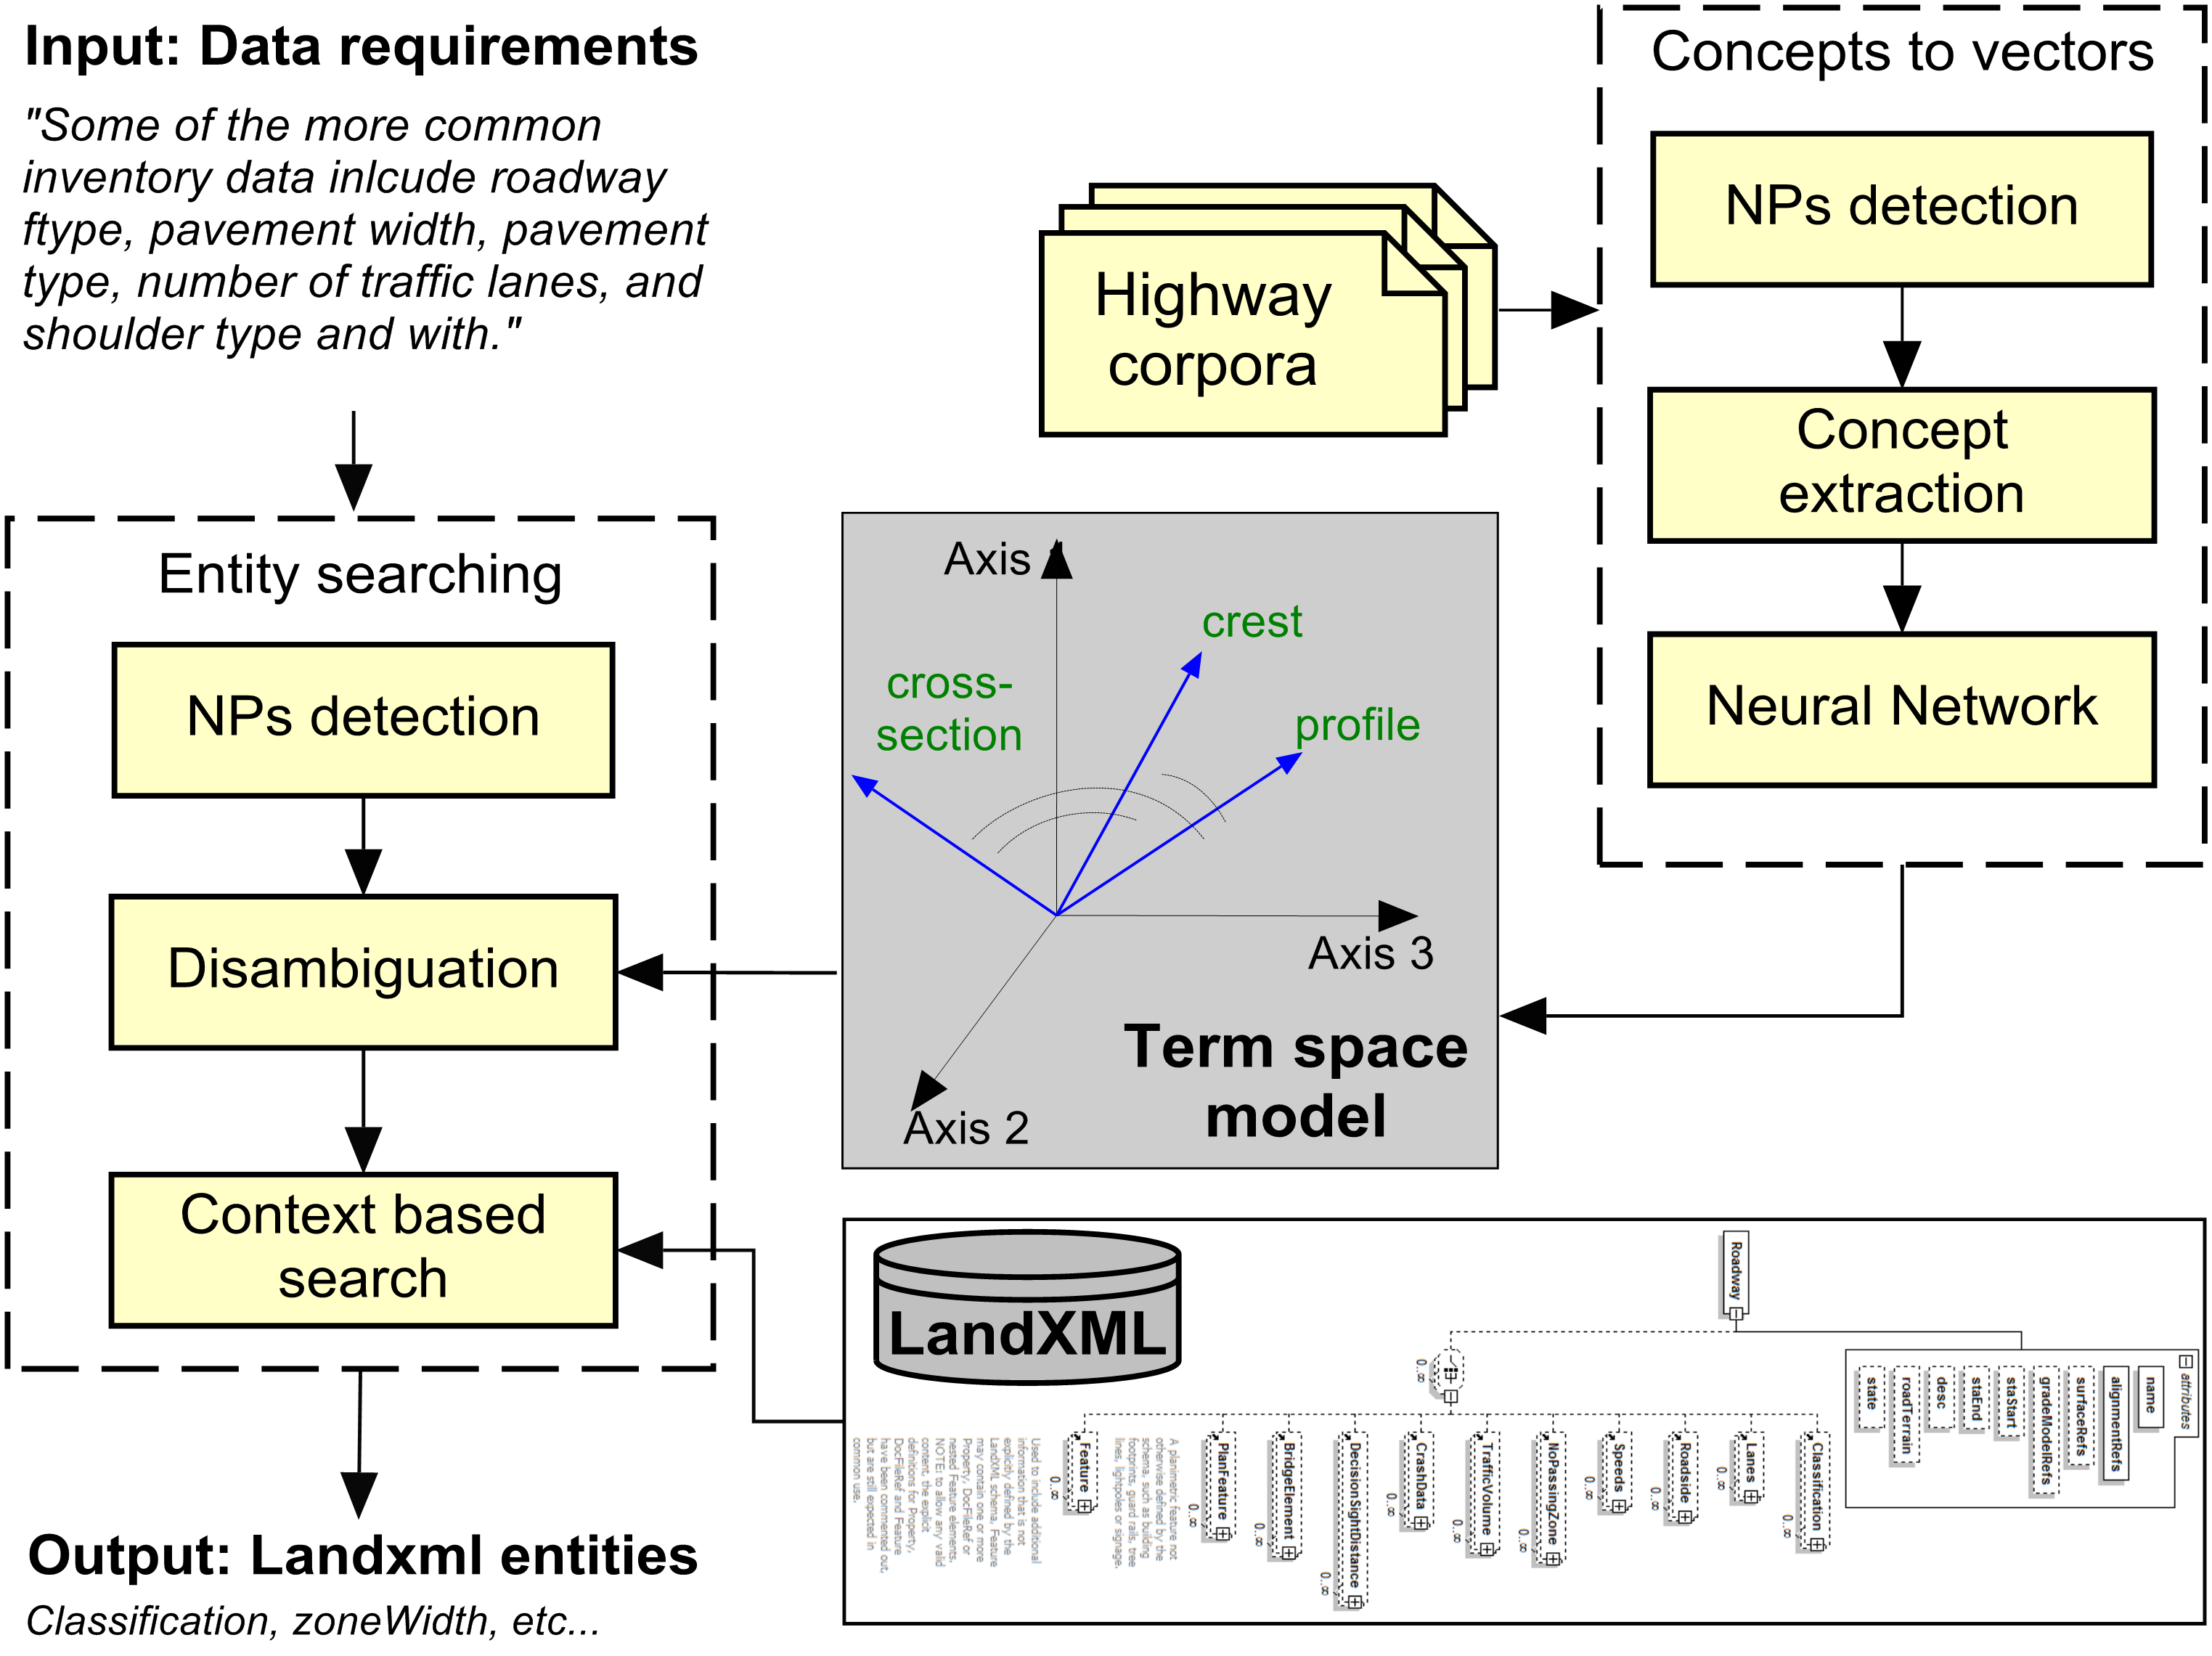
\includegraphics[width=0.67\textwidth]{framework3}
\caption{Overall architecture for automated generation of MDV}
\label{fig:framework}
\end{figure}
%
Figure \ref{fig:framework} presents the proposed framework for automated generation of model views. The framework is consisted of two components that are: (1) a highway term space model, and (2) a semantic searching algorithm. The first module aims to extract highway related technical concepts from the highway corpora and transform concepts into vectors representing their meanings by employing a neural network (NN) model and a set of NLP techniques. Using this concept vector space, synonyms or associated concepts can be determined based on the distance or angle between vectors. The purpose of the second module is to semantically search for LandXML entities and attributes based on the natural language data requirement inputs. In order to achieve this objective, NLP techniques firstly are applied on the natural language data requirements to extract keywords that representing what types of data needed to be transferred to the data receiver. A proposed algorithm then is utilized to disambiguate the meaning of extracted required data keywords based on the term space model and search for equivalent entities or attributes included in the LandXML data schema. The following sections respectively presents the process of building the highway term space model and the searching algorithm along with details on which methods/tools utilized 
%
\section{Highway term space model} \label{sec:vector-space}
%
%introduction to the distributional vector model, fundamental theory,  the overall process to translate technical terms into vectors representations. the role of vector space allow measure the similarity between 
The ultimate goal of this module is to building a model that can support the disambiguation task. For disambiguation, there are several methods including thesaurus based, ontology based and distributional method. The first two methods required a full lexicon or ontology including concepts description for all aspects/disciplines in the highway industry. These methods would be ideal for the disambiguation task if domain related thesauruses are available. However, since building up those dictionaries required a huge amount of empirical work, they are still limited. Wordnet \cite{Miller95} which is one of the largest lexicons available containing 117,000 synsets, but it is generic and is not suitable for the highway domain. For this reason, this research employs the distribution method which is based on an unsupervised machine learning method to train unlabeled data and learn the meaning of words by analyzing the context of words.
\par
Highway vector space model (H-VSM) is one of the key results of this research. The skip-gram model, proposed by \citeN{Mikolov13a}, which is a neural network (NN) model was employed to develop the H-VSM. The NN model was designed to predict the context words of a given word included in the input corpora. The sub-sections below present the detailed procedure followed to collect input data which is the highway domain corpora and utilize the skip-gram model to convert highway technical concepts to vectors.
%
\subsection{Data collection}
%how to collect data, how to clean data to get them readay for training model
%aim text folow remained, flow direction. bottom down, 
%remove heading (chapter, section, subsection), footnote, numerbing, bullets, hyperlink, url, 
Highway corpus was collected from a number of documents from multiple sources including textbooks, and highway engineering manuals from federal Department of Transportation and from 18 state DOTs. The focus of highway corpora in this this research were on three  project phases including design, construction and asset management. Since technical guidance documents in the engineering field contains a variety of text formats such as text, tables, equations. The order of words in tables and equations are not structured in the sentence format, their words are not suitable for the training process. Hence, these tables were removed from the text corpora. The result of the data collection was a highway corpora consisting of 10 millions words. This data set was utilized to extract highway related technical terms which were then trained and converted into vectors. 
\subsection{Concept extraction}
%introduction to concept extraction

\begin{figure}[t]
\centering
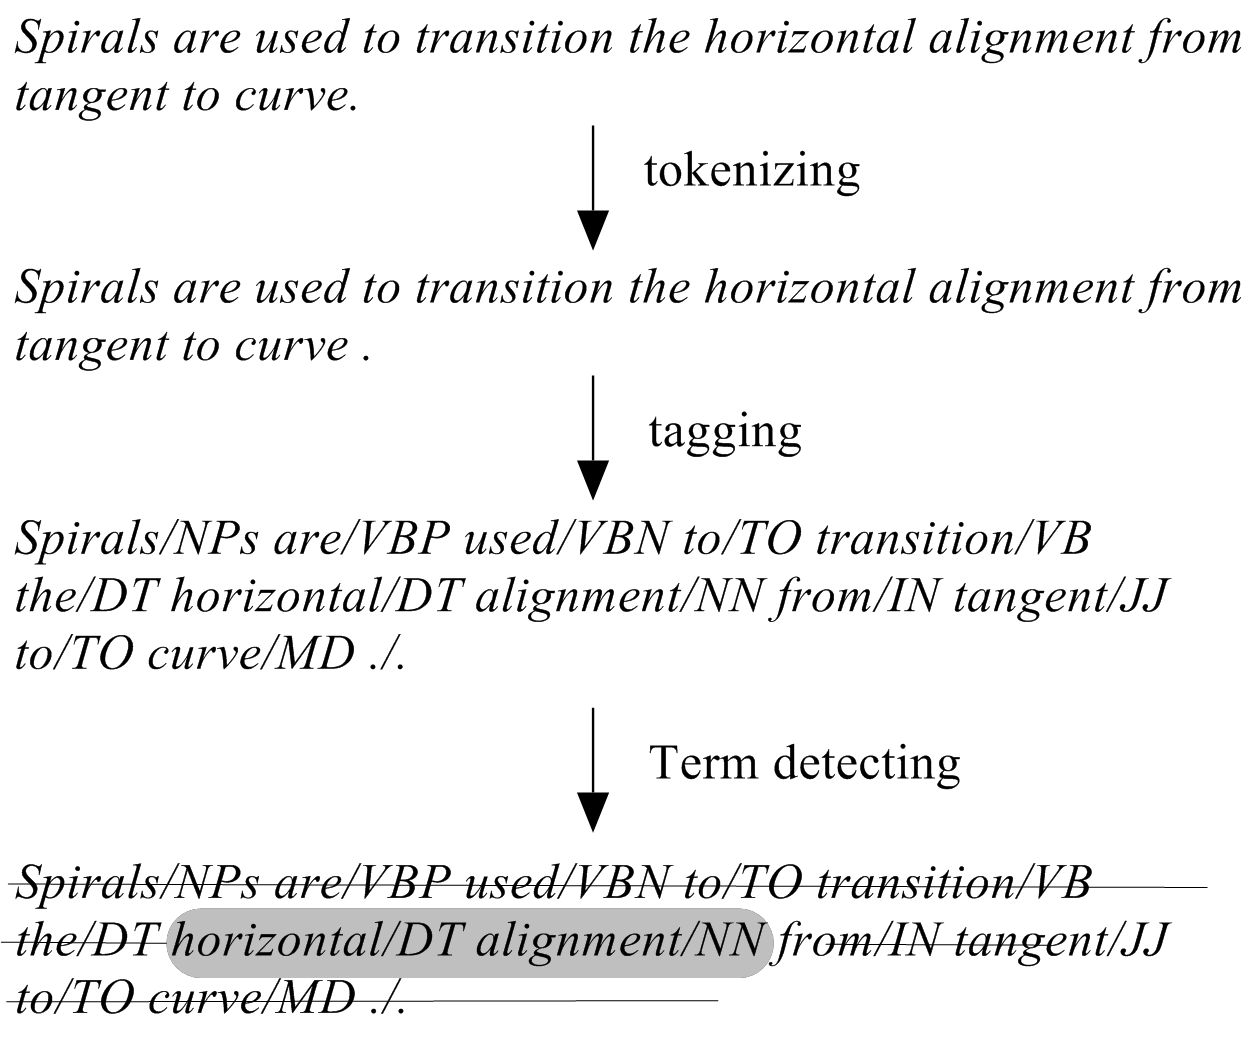
\includegraphics[width=0.45\textwidth]{NP_detecting}
\caption{Linguistic processing procedure to detect technical terms}
\label{fig:np_detect}
\end{figure}
%brief introduction about data requirements, and the purposes of this module

The first step in building the H-VSM is the identifying of highway related technical concepts. In order to achieve this task, a set of natural language processing techniques including tokenization, part of speech tagging were utilized to identify the POS tag for each word in the highway corpora. The OpenNLP library was used to perform this task. The linguistic process, as illustrated in the Figure \ref{fig:np_detect}, includes the following steps:

\subsubsection{Word Tokenization} 
In this step, text was broken down into individual units (called tokens). 
\subsubsection{POS tagging} 
The purpose of this step is to determine the part of speech tag for each token. 
\subsubsection{Noun phrase detection}
For this task, any phrases having either the following patterns (A|N)1*N1 Prep(of) (A|N)2*N2 or (A|N)1*N1(A|N)2N2 are categorized as noun phrases and are good candidates for technical terms. In the patterns above, A is adjective and N is noun. 
\subsubsection{Termhood measurement and concept extraction}
The C-Value algorithm, proposed by \cite{Frantzi20} was employed to extract technical concepts. The idea of the C-value method is to firstly extract noun phrases which are composed of adjective and nouns, and then measure the how frequent they occur in the corpus. Equation below presents the C-value measurement of termhood.

\begin{equation}
    C-value(a)=
    \begin{cases}
      log_2|a|.f(a), & \text{if a is not nested} \\
      log_2|a|(f(a)-\frac{1}{P(T_a)}\sum_{b\in T_a} f(b)), & \text{otherwise}
    \end{cases}
  \end{equation}
  
where:
\begin{description}
\item[a] is a candidate noun phrase
\item[f] is the frequency of a in the corpus
\item[Ta] is the set of extracted noun phrases that contains a
\item[P(Ta)] is the number of these candidate terms.
\end{description}

\begin{figure}[t]
\centering
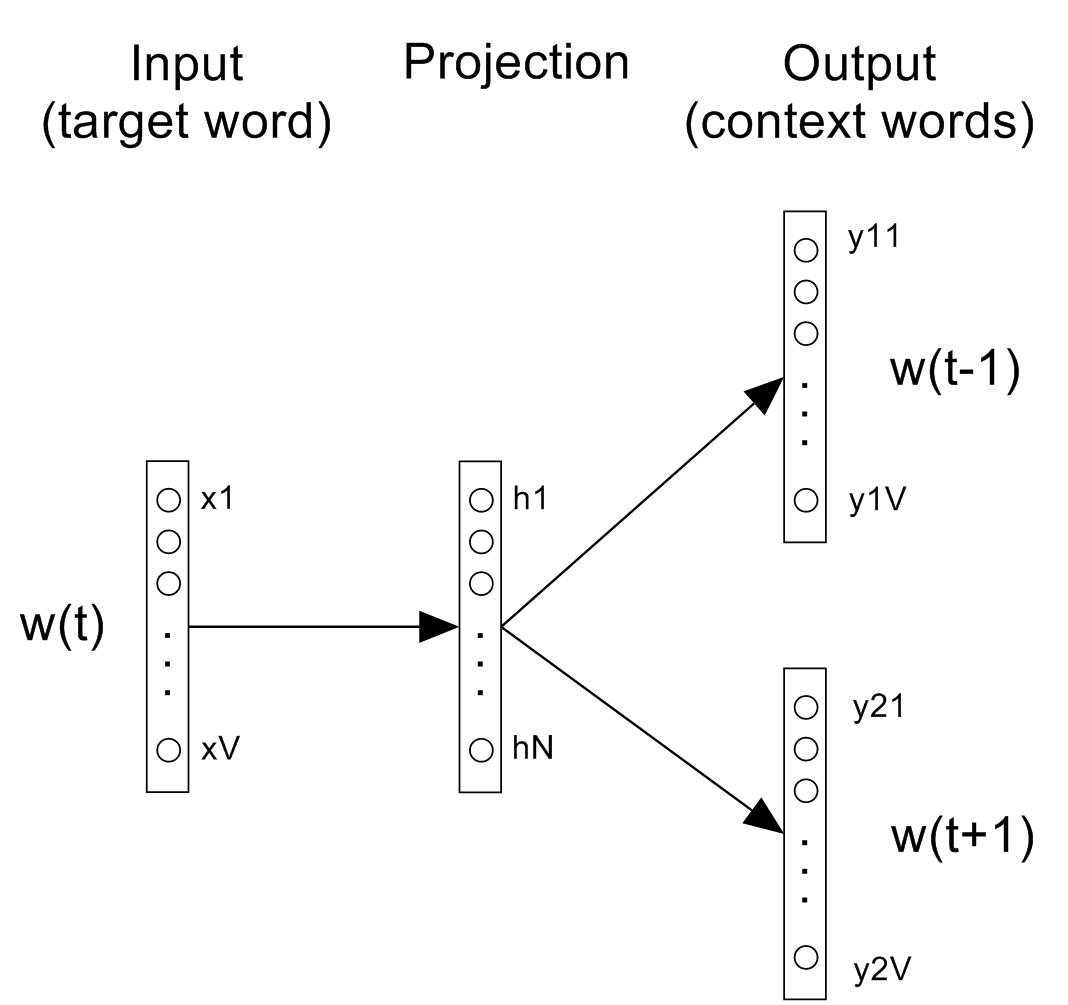
\includegraphics[width=0.45\textwidth]{skip-gram-model}
\caption{Skip-gram model}
\label{fig:skip-gram}
\end{figure}

\subsection{Data training}
%word2vec, brief introduction about word2vec
%skip-gram model
%how to modify the method of selecting conext words
%java program
This research employed the skip-gram neural network training model which was developed by \cite{Mikolov13a} to train the highway corpus.  The distributional hypothesis is the fundamental theory of this method. The distributional hypothesis says that two words have the same meanings if they occur in the same contexts \cite{harispe15}. For example, ``apple'' is more similar to ``banana''  than coffee since ``apple'' and ``banana'' are both co-occur with the word ``eat'', while ``coffee'' more frequently co-occur with the word ``drink''. Figure \ref{fig:skip-gram} presents the architecture of the skip-gram model. The model includes 3 layers including input, hidden and output layer. The input data is the target word and the output data are the context words surrounding the target word. Each word in the vocabulary set (with the size V) is encoded into one-hot vector in which only the value at the word index is equal to one and other positions are zero. In order to train the model, the java library word2vec, developed by Google was used. The parameters of the model, as presented in Table \ref{table:nn-parameters}, were selected based on the suggestions in the literature.
%


\begin{table} [t]
\caption{Skip-gram model parameters}
\label{table:nn-parameters}
\centering
\small
\renewcommand{\arraystretch}{1.25}
\begin{tabular}{l l}
\hline
\textbf{Parameter} & \textbf{Value}\\

\hline
Hidden size		&	300\\
Window size	&	15\\

\hline
\end{tabular}
\normalsize
\end{table}

\section{Context based searching algorithm} \label{sec:searching}
This section presents the proposed algorithm (see Figure \ref{fig:search_algorithm}) for semantically searching for equivalent entities/attributes in Landxml schema. The algorithm is a three-stage procedure. In the the first stage, a list of synonym concepts that have the similar meanings to the keyword input are generated by utilizing the vector space model developed above. Each synonym concept is defined by their attributes. A string based searching is then applied to find the entity in the Landxml schema that has the most similar name for each synonym in the list. Any synonym that match to at least one Landxml entity in this phase is considered as potential candidate. These candidates are then tested in the final phase. Concepts which fail the testing phase are removed from the candidate list. The test is to examine if the synonym and it's matched entity share the same attributes. If two objects are similar, they would share common attributes. The final matches are ranked by the similarity score. 

%\subsection{Term disambiguation}

%\subsection{Semantics based searching algorithm}

\begin{figure}[t]
\centering
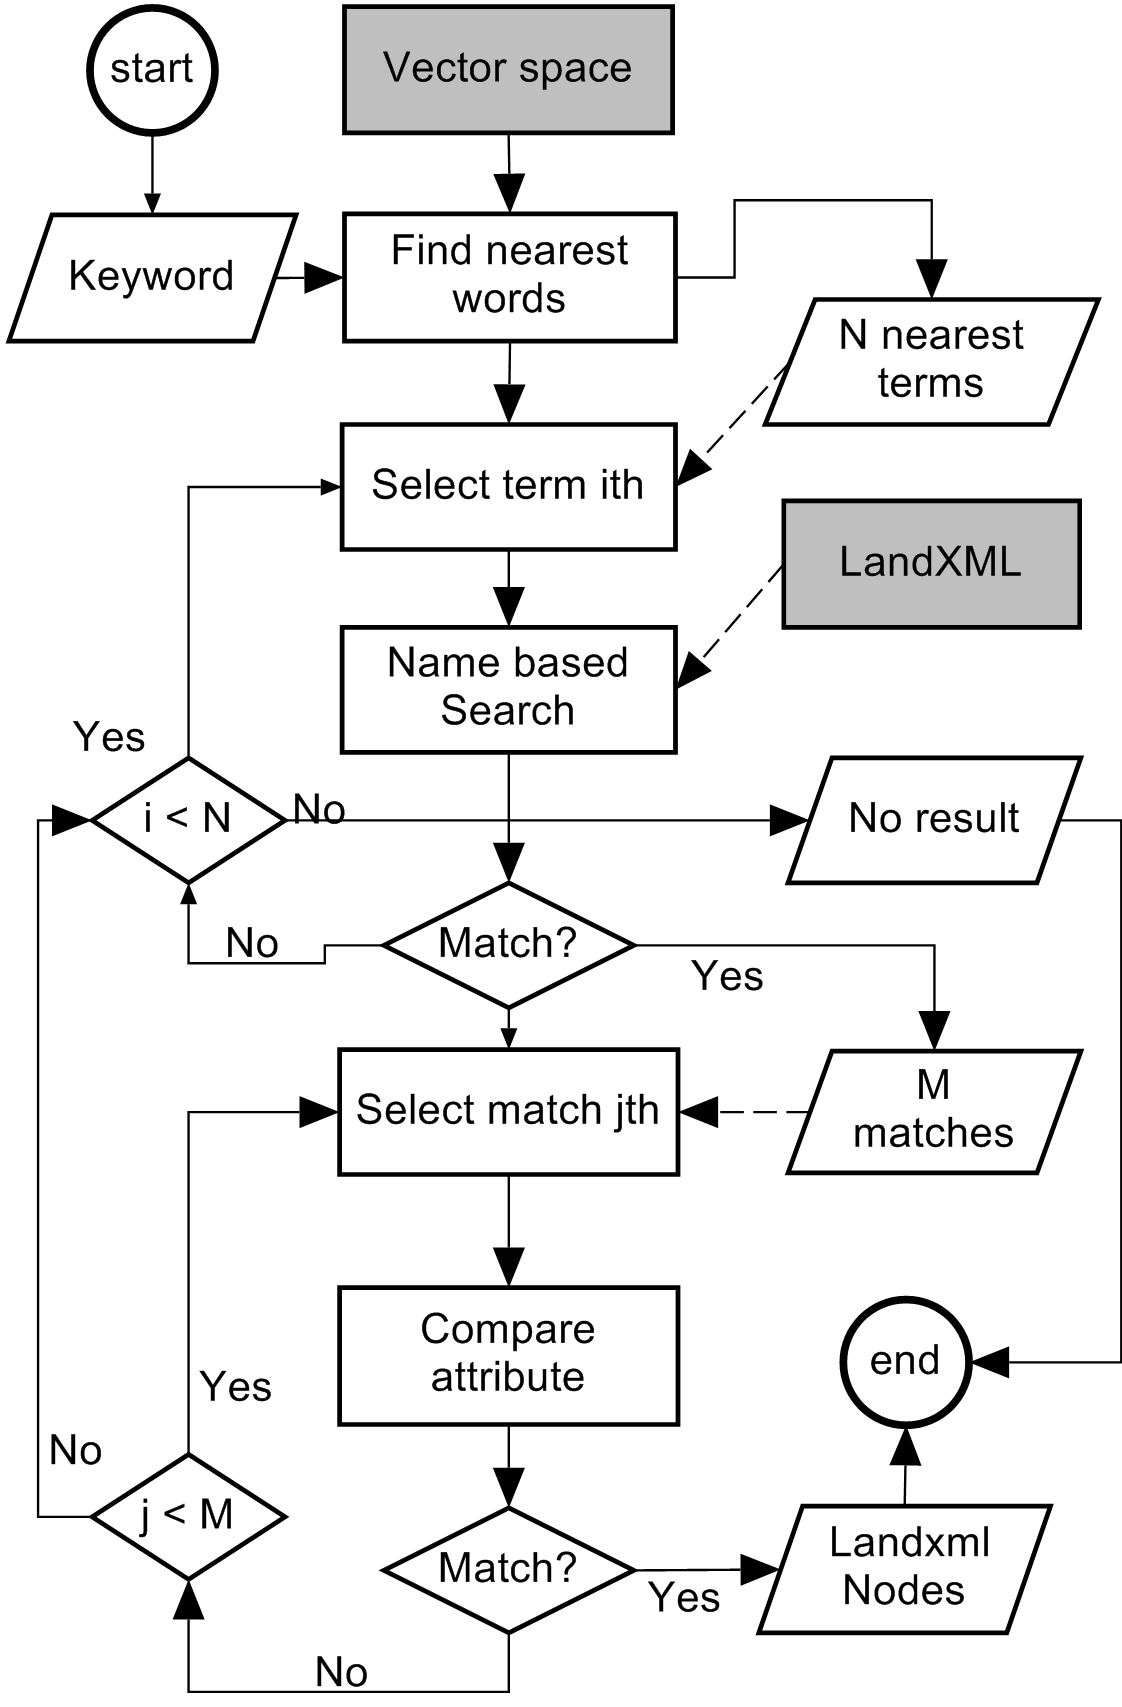
\includegraphics[width=0.45\textwidth]{entity_search_algorithm}
\caption{Entity searching algorithm}
\label{fig:search_algorithm}
\end{figure}

\section{Evaluation} \label{sec:val}
An evaluation experiment was conducted to evaluate the context-aware searching algorithm. In this experiment, a graduate student was asked to read a randomly selected document which contains data requirements for a specific data transaction. The duty of the student was to manually identify a set of Landxml entities that would fulfill the data requirements. Meanwhile, a prototype built upon the developed algorithm was applied to automatically generate the subset of data from the same document as the student used. The results from the two methods were used to calculate the accuracy of the searching algorithm.
%
\begin{align} 
&Recall = \frac{\text{number of correctly matched concepts}}{\text{total concepts}}  \\ 
&Precision = \frac{\text{number of correctly matched concepts}}{\text{total matched concepts}}  \\
&F-measure = \frac{2.Precision.Recall}{Precision+Recall}
\end{align}
%
\begin{table} [b] 
\caption{Evaluation result}
\label{table:eva}
\centering
\small
\renewcommand{\arraystretch}{1.25}
\begin{tabular}{l l l l l l}


\hline
\hline
 Tested concepts & Matched concepts & Correct & Recall(\%) & Precision (\%) & F (\%)\\
 \hline
23 & 21 & 19 & 82 & 90 & 84\\


\hline
\hline
\end{tabular}
\normalsize
\end{table}


\begin{table} [t] 
\caption{Matching examples}
\label{table:examples}
\centering
\small
\renewcommand{\arraystretch}{1.25}
\begin{tabular}{l l l l}
\hline
\hline
\textbf{Keyword} & \textbf{Matched Landxml entities} & \textbf{Score} & \textbf{Correct?}\\
\hline
drainage system & Outlet & 1.00 & yes\\
 & OutletStruct & 0.46\\
Vertical alignment & roadTerrain & 0.58 & no\\
 & pointGeometry & 0.57\\
pavement type & pavementSurfaceType & 0.19 & yes\\
 & stateType & 0.18\\
 & projectType & 0.15\\
shoulder & sidewalk & 1.00\\
 & road shoulder & 0.61 & yes\\
roadway type & classification & 0.56 & yes\\
 & RoadSign type & 0.44\\
aadt & ADT & 1.00 & yes\\
\hline
\hline
\end{tabular}
\normalsize
\end{table}
%
Table \ref{table:eva} shows the evaluation result. As presented in the table, the system shows a 90 percent precision. However, the recall is relatively low accuracy, this is possibly due to the the training data size. Since the searching algorithm accuracy is highly rely on the a capacity of finding synonyms which is based on the vector space model. This model currently is based on the data training set consisting of only 10 million words. In order to enhance the accuracy, the data training set needs to be extended. Future research will be conducted to extend the training data set. 
%
\section{Conclusions} \label{sec:conclns} 
Digital data has been widely generated through the project life cycle. However, the data collected and generated in previous stages are no reusable in the downstream phases. This issue is due to the interoperability when digital data from one partner is not readable or correctly understandable by the data receiver. This research develops an framework that semantically searches for desired data from the transferred data file. The framework is composed of two components including (1) a terms space model which represents highway related concepts extracted from the highway corpora in vectors and (2) a context based searching algorithm that can search for entities in the Landxml schema based on their similarity of attributes instead of string based similarity. 
\par
The framework has been evaluated by testing on a randomly selected set of input data. The result shows the accuracy of over 80 percent. The accuracy is low due to the size of the training data. Future research will be conducted to increase the data size. 
\par
This method is broad and can be applied to other business processes such as green building checking, environment checking, etc. The method is expected to significantly improve the existing ad-hoc method of model view definition development and in return leads the the removal of this bottle neck which is restricting the seamless data integration and exchange across phases of a highway construction project. 

%bibliography
\bibliography{bibliography}
%
%
\end{document}

